\documentclass{article}

% content/resources/templates/preamble.tex
\usepackage[margin=0.6in]{geometry}
\author{Milav Dabgar}
\usepackage{amsmath,amssymb,amsthm}
\usepackage{booktabs}
\usepackage{multirow}
\usepackage{xcolor}
\usepackage{tcolorbox}
\tcbuselibrary{breakable,skins}
\usepackage[colorlinks=true,linkcolor=blue]{hyperref}
\usepackage{titlesec}
\usepackage{enumitem}
\usepackage{tikz}
\usepackage{pgfplots}
\usepackage{circuitikz}
\usepackage[version=4]{mhchem}
\usepackage{longtable}
\usepackage{array}
\usepackage{float}
\usepackage{caption}
\usepackage{listings}

\lstset{
  basicstyle=\small\ttfamily,
  breaklines=true,
  breakatwhitespace=false,
  postbreak=\mbox{\textcolor{red}{$\hookrightarrow$}\space},
  float=false,
  numbers=left,
  numberstyle=\tiny\color{gray},
  numbersep=10pt,
  xleftmargin=2em,
  keywordstyle=\color{blue},
  commentstyle=\color{green!60!black},
  stringstyle=\color{purple},
  backgroundcolor=\color{gray!5},
  showstringspaces=false,
  tabsize=2,
  captionpos=b,
  keepspaces=true,
  columns=flexible
}

\pgfplotsset{compat=1.18}
\usetikzlibrary{shapes,arrows,positioning,calc,patterns,decorations.pathmorphing,decorations.markings,arrows.meta}

% Color scheme
\definecolor{headcolor}{RGB}{0,102,204}
\definecolor{keycolor}{RGB}{220,20,60}
\definecolor{solutioncolor}{RGB}{34,139,34}
\definecolor{mnemoniccolor}{RGB}{148,0,211}
\definecolor{codecolor}{RGB}{0,0,100}

% Spacing
\setlength{\parskip}{3pt}
\setlist[itemize]{nosep}
\setlist[enumerate]{nosep}

% Title formatting
\titleformat{\section}{\Large\bfseries\color{headcolor}}{\thesection}{1em}{}
\titleformat{\subsection}{\large\bfseries\color{headcolor}}{\thesubsection}{1em}{}

% Pandoc tightlist compatibility
\providecommand{\tightlist}{%
  \setlength{\itemsep}{0pt}\setlength{\parskip}{0pt}}

% Pandoc longtable compatibility
\newcounter{none}
\def\thenone{}


% content/resources/templates/english-boxes.tex

% Custom environments
\newtcolorbox{solutionbox}{
 breakable,
 enhanced,
 colback=solutioncolor!5!white,
 colframe=solutioncolor!75!black,
 fonttitle=\bfseries,
 title=Solution
}

\newtcolorbox{solutionboxnobreak}{
 colback=solutioncolor!5!white,
 colframe=solutioncolor!75!black,
 fonttitle=\bfseries,
 title=Solution
}

\newtcolorbox{keyformula}{
 breakable,
 enhanced,
 colback=keycolor!5!white,
 colframe=keycolor!75!black,
 fonttitle=\bfseries,
 title=Key Formula
}

\newtcolorbox{mnemonicboxenv}{
 breakable,
 enhanced,
 colback=mnemoniccolor!5!white,
 colframe=mnemoniccolor!75!black,
 fonttitle=\bfseries,
 title=Mnemonic
}

\newcommand{\mnemonicbox}[1]{%
  \begin{mnemonicboxenv}
    #1
  \end{mnemonicboxenv}
}


% Custom commands for GTU solutions
% This file defines semantic commands for consistent formatting

% Question command with automatic formatting
\newcommand{\question}[2]{%
  \section*{Question #1}%
  \textbf{#2}%
}

% OR question variant
\newcommand{\questionor}[2]{%
  \section*{Question #1 OR}%
  \textbf{#2}%
}

% Proper table environment with caption
\newenvironment{answertable}[1]{%
  \begin{table}[htbp]
  \centering
  \caption{#1}
}{%
  \end{table}
}

% Proper figure environment for diagrams
\newenvironment{answerdiagram}[1]{%
  \begin{figure}[htbp]
  \centering
  \caption{#1}
}{%
  \end{figure}
}

% Semantic markup for key terms
\newcommand{\keyword}[1]{\textbf{#1}}
\newcommand{\code}[1]{\texttt{#1}}
\newcommand{\classname}[1]{\texttt{#1}}
\newcommand{\methodname}[1]{\texttt{#1}}

% Proper quotation marks
\newcommand{\mnemonic}[1]{``#1''}

\usetikzlibrary{shapes.multipart, chains, arrows.meta, positioning, calc, trees}

\title{Data Structure And Application (1333203) - Summer 2025 Solution}
\date{May 15, 2025}

\begin{document}
\maketitle

\questionmarks{1(a)}{3}{Define Big - O Notation, Big Omega Notation, Big Theta Notation.}

\begin{solutionbox}
\begin{center}
\captionof{table}{Asymptotic Notations Comparison}
\begin{tabulary}{\linewidth}{|L|L|L|L|}
\hline
\textbf{Notation} & \textbf{Symbol} & \textbf{Description} & \textbf{Usage} \\ \hline
Big-O & $O(f(n))$ & Upper bound & Worst case \\ \hline
Big Omega & $\Omega(f(n))$ & Lower bound & Best case \\ \hline
Big Theta & $\Theta(f(n))$ & Tight bound & Average case \\ \hline
\end{tabulary}
\end{center}

\begin{itemize}
    \item \textbf{Big-O Notation}: Describes maximum time/space complexity
    \item \textbf{Big Omega}: Describes minimum time/space complexity
    \item \textbf{Big Theta}: Describes exact time/space complexity
\end{itemize}
\end{solutionbox}

\begin{mnemonicbox}
\mnemonic{OWT - O for wOrst, Omega for Best, Theta for Tight}
\end{mnemonicbox}

\questionmarks{1(b)}{4}{Define Set. Write various operations that can be performed on Set.}

\begin{solutionbox}
\textbf{Definition}: Set is a collection of unique elements with no duplicates.

\begin{center}
\captionof{table}{Set Operations}
\begin{tabulary}{\linewidth}{|L|L|L|L|}
\hline
\textbf{Operation} & \textbf{Symbol} & \textbf{Description} & \textbf{Example} \\ \hline
Union & $A \cup B$ & Combines all elements & $\{1,2\} \cup \{2,3\} = \{1,2,3\}$ \\ \hline
Intersection & $A \cap B$ & Common elements & $\{1,2\} \cap \{2,3\} = \{2\}$ \\ \hline
Difference & $A - B$ & Elements in A not in B & $\{1,2\} - \{2,3\} = \{1\}$ \\ \hline
Subset & $A \subseteq B$ & All A elements in B & $\{1\} \subseteq \{1,2\} = True$ \\ \hline
\end{tabulary}
\end{center}

\begin{itemize}
    \item \textbf{Add/Insert}: Adding new element
    \item \textbf{Remove/Delete}: Removing existing element
    \item \textbf{Contains}: Check if element exists
\end{itemize}
\end{solutionbox}

\begin{mnemonicbox}
\mnemonic{UIDS - Union, Intersection, Difference, Subset}
\end{mnemonicbox}

\questionmarks{1(c)}{7}{Write a Python class to represent a Cricketer. The class contains the name of the cricketer, team name and run as the data members. The member functions are as follows: to initialize the data members, to set run and display run.}

\begin{solutionbox}
\begin{lstlisting}[language=Python]
class Cricketer:
    def __init__(self, name="", team="", run=0):
        self.name = name
        self.team = team
        self.run = run
    
    def set_run(self, run):
        self.run = run
    
    def display_run(self):
        print(f"Player: {self.name}")
        print(f"Team: {self.team}")
        print(f"Runs: {self.run}")

# Example usage
player = Cricketer("Virat Kohli", "India", 100)
player.display_run()
\end{lstlisting}

\begin{itemize}
    \item \textbf{Constructor}: Initializes name, team, and run
    \item \textbf{set\_run()}: Updates run value
    \item \textbf{display\_run()}: Shows player information
\end{itemize}

\begin{center}
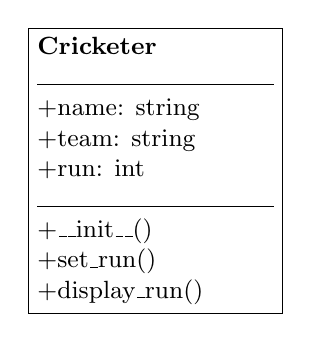
\begin{tikzpicture}[class/.style={rectangle, draw, minimum width=3cm, align=left, font=\small}]
    \node [class] (cricketer) {
        \textbf{Cricketer} \\
        \rule{3cm}{0.5pt} \\
        +name: string \\
        +team: string \\
        +run: int \\
        \rule{3cm}{0.5pt} \\
        +\_\_init\_\_() \\
        +set\_run() \\
        +display\_run()
    };
\end{tikzpicture}
\captionof{figure}{Cricketer Class Diagram}
\end{center}
\end{solutionbox}

\begin{mnemonicbox}
\mnemonic{CSD - Constructor, Set, Display}
\end{mnemonicbox}

\questionmarks{1(c) OR}{7}{Design a student class for reading and displaying the student information, the getInfo() and displayInfo() methods will be used respectively. Where getInfo() will be a private method.}

\begin{solutionbox}
\begin{lstlisting}[language=Python]
class Student:
    def __init__(self):
        self.name = ""
        self.roll_no = ""
        self.marks = 0
        self.__getInfo()  # Private method call
    
    def __getInfo__(self):  # Private method
        self.name = input("Enter name: ")
        self.roll_no = input("Enter roll number: ")
        self.marks = int(input("Enter marks: "))
    
    def displayInfo(self):
        print(f"Name: {self.name}")
        print(f"Roll No: {self.roll_no}")
        print(f"Marks: {self.marks}")

# Example usage
student = Student()
student.displayInfo()
\end{lstlisting}

\begin{itemize}
    \item \textbf{Private method}: Uses double underscore (\_\_getInfo)
    \item \textbf{Constructor}: Automatically calls private method
    \item \textbf{Public method}: displayInfo() shows student data
\end{itemize}
\end{solutionbox}

\begin{mnemonicbox}
\mnemonic{PCP - Private, Constructor, Public}
\end{mnemonicbox}

\questionmarks{2(a)}{3}{Differentiate between Stack and Queue.}

\begin{solutionbox}
\begin{center}
\captionof{table}{Stack vs Queue Comparison}
\begin{tabulary}{\linewidth}{|L|L|L|}
\hline
\textbf{Feature} & \textbf{Stack} & \textbf{Queue} \\ \hline
Order & LIFO (Last In First Out) & FIFO (First In First Out) \\ \hline
Operations & Push, Pop & Enqueue, Dequeue \\ \hline
Access Point & One end (top) & Two ends (front \& rear) \\ \hline
Example & Plates stack & Bank queue \\ \hline
\end{tabulary}
\end{center}

\begin{center}
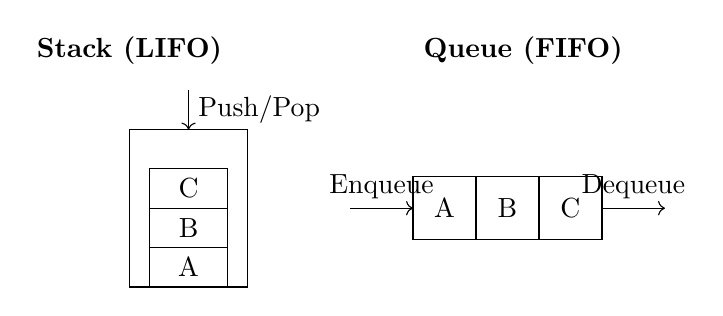
\begin{tikzpicture}[
    stacknode/.style={rectangle, draw, minimum width=1cm, minimum height=0.5cm},
    queuenode/.style={rectangle, draw, minimum width=0.8cm, minimum height=0.8cm}
]
    % Stack Visualization
    \node (slabel) at (0, 3) {\textbf{Stack (LIFO)}};
    \draw (0,0) -- (0,2) -- (1.5,2) -- (1.5,0) -- cycle;
    \node[stacknode] at (0.75, 0.25) {A};
    \node[stacknode] at (0.75, 0.75) {B};
    \node[stacknode] at (0.75, 1.25) {C};
    \draw[->] (0.75, 2.5) -- node[right] {Push/Pop} (0.75, 2.0);

    % Queue Visualization
    \node (qlabel) at (5, 3) {\textbf{Queue (FIFO)}};
    \node[queuenode] (q1) at (4, 1) {A};
    \node[queuenode] (q2) at (4.8, 1) {B};
    \node[queuenode] (q3) at (5.6, 1) {C};
    \draw (3.6, 1.4) -- (6.0, 1.4);
    \draw (3.6, 0.6) -- (6.0, 0.6);
    \draw[<-] (3.6, 1) -- node[above] {Enqueue} (2.8, 1);
    \draw[->] (6.0, 1) -- node[above] {Dequeue} (6.8, 1);
\end{tikzpicture}
\captionof{figure}{Stack and Queue Structure}
\end{center}
\end{solutionbox}

\begin{mnemonicbox}
\mnemonic{SLIF QFIF - Stack LIFO, Queue FIFO}
\end{mnemonicbox}

\questionmarks{2(b)}{4}{Define recursion. Explain with example.}

\begin{solutionbox}
\textbf{Definition}: Function calling itself with smaller problem until base condition.

\begin{lstlisting}[language=Python]
def factorial(n):
    # Base case
    if n <= 1:
        return 1
    # Recursive case
    return n * factorial(n-1)

# Example: factorial(3)
# 3 * factorial(2)
# 3 * 2 * factorial(1)
# 3 * 2 * 1 = 6
\end{lstlisting}

\begin{itemize}
    \item \textbf{Base case}: Stopping condition
    \item \textbf{Recursive case}: Function calls itself
    \item \textbf{Problem reduction}: Each call handles smaller problem
\end{itemize}
\end{solutionbox}

\begin{mnemonicbox}
\mnemonic{BRP - Base, Recursive, Problem-reduction}
\end{mnemonicbox}

\questionmarks{2(c)}{7}{Consider the size of the stack as 5. Apply the following operation on stack and show status and top pointer after each operation. Push a,b,c pop}

\begin{solutionbox}
\textbf{Stack Operations Trace:}

\begin{center}
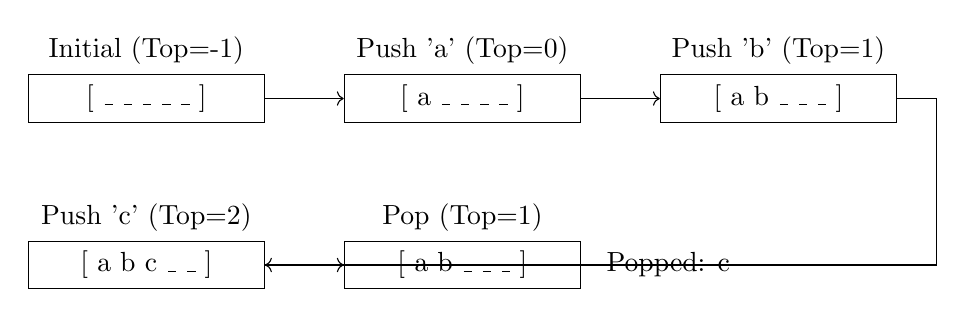
\begin{tikzpicture}[
    stackbox/.style={rectangle, draw, minimum width=3cm, minimum height=0.6cm, align=center},
    pointer/.style={->, thick, red}
]
    % Initial
    \node[stackbox] (s0) at (0,0) {[ \_ \_ \_ \_ \_ ]};
    \node[above] at (s0.north) {Initial (Top=-1)};

    % Push a
    \node[stackbox, right=1cm of s0] (s1) {[ a \_ \_ \_ \_ ]};
    \node[above] at (s1.north) {Push 'a' (Top=0)};

    % Push b
    \node[stackbox, right=1cm of s1] (s2) {[ a b \_ \_ \_ ]};
    \node[above] at (s2.north) {Push 'b' (Top=1)};
    
    % Push c
    \node[stackbox, below=1.5cm of s0] (s3) {[ a b c \_ \_ ]};
    \node[above] at (s3.north) {Push 'c' (Top=2)};
    
    % Pop
    \node[stackbox, right=1cm of s3] (s4) {[ a b \_ \_ \_ ]};
    \node[above] at (s4.north) {Pop (Top=1)};
    \node[right=0.2cm of s4] {Popped: c};

    % Arrows
    \draw[->] (s0) -- (s1);
    \draw[->] (s1) -- (s2);
    \draw[->] (s2.east) -- ++(0.5,0) |- (s3.east);
    \draw[->] (s3) -- (s4);

\end{tikzpicture}
\captionof{figure}{Stack Operations Trace}
\end{center}

\begin{itemize}
    \item \textbf{Push operations}: Add elements from index 0 onwards
    \item \textbf{Top pointer}: Points to last inserted element
    \item \textbf{Pop operation}: Removes top element, decrements top pointer
\end{itemize}
\end{solutionbox}

\begin{mnemonicbox}
\mnemonic{PTD - Push Top Decrement}
\end{mnemonicbox}

\questionmarks{2(a) OR}{3}{List applications of Stack and Queue.}

\begin{solutionbox}
\begin{center}
\captionof{table}{Applications of Stack and Queue}
\begin{tabulary}{\linewidth}{|L|L|}
\hline
\textbf{Data Structure} & \textbf{Applications} \\ \hline
\textbf{Stack} & Function calls, Undo operations, Expression evaluation, Browser history \\ \hline
\textbf{Queue} & Process scheduling, Printer queue, BFS traversal, Handling requests \\ \hline
\end{tabulary}
\end{center}
\end{solutionbox}

\begin{mnemonicbox}
\mnemonic{Stack FUBE, Queue SPBH}
\end{mnemonicbox}

\questionmarks{2(b) OR}{4}{Convert following algebraic expression into postfix notation using Stack: i) (a*b)*(c\textasciicircum d(d+e)-f) ii) a-b/(c*d/e)}

\begin{solutionbox}
\textbf{i) $(a*b)*(c\textasciicircum d(d+e)-f)$}

\begin{center}
\small
\begin{tabulary}{\linewidth}{|L|L|L|}
\hline
\textbf{Symbol} & \textbf{Stack} & \textbf{Output} \\ \hline
( & ( & \\ \hline
a & ( & a \\ \hline
* & (* & a \\ \hline
b & (* & ab \\ \hline
) & & ab* \\ \hline
* & * & ab* \\ \hline
( & *( & ab* \\ \hline
c & *( & ab*c \\ \hline
\textasciicircum & *(\textasciicircum & ab*c \\ \hline
d & *(\textasciicircum & ab*cd \\ \hline
( & *(\textasciicircum( & ab*cd \\ \hline
d & *(\textasciicircum( & ab*cdd \\ \hline
+ & *(\textasciicircum(+ & ab*cdd \\ \hline
e & *(\textasciicircum(+ & ab*cdde \\ \hline
) & *(\textasciicircum & ab*cdde+ \\ \hline
) & * & ab*cdde+\textasciicircum \\ \hline
- & *- & ab*cdde+\textasciicircum \\ \hline
f & *- & ab*cdde+\textasciicircum f \\ \hline
& & ab*cdde+\textasciicircum f-* \\ \hline
\end{tabulary}
\end{center}
\textbf{Result:} $ab*cdde+\textasciicircum f-*$

\textbf{ii) $a-b/(c*d/e)$}

\textbf{Result:} $abcd*e/-$
\end{solutionbox}

\begin{mnemonicbox}
\mnemonic{PEMDAS reversed for postfix}
\end{mnemonicbox}

\questionmarks{2(c) OR}{7}{Develop a program to implement a queue using a list that performs following operations: enqueue, dequeue.}

\begin{solutionbox}
\begin{lstlisting}[language=Python]
class Queue:
    def __init__(self):
        self.queue = []
        self.front = 0
        self.rear = -1
    
    def enqueue(self, item):
        self.queue.append(item)
        self.rear += 1
        print(f"Enqueued: {item}")
    
    def dequeue(self):
        if self.front <= self.rear:
            item = self.queue[self.front]
            self.front += 1
            print(f"Dequeued: {item}")
            return item
        else:
            print("Queue is empty")
            return None
    
    def display(self):
        if self.front <= self.rear:
            print("Queue:", self.queue[self.front:self.rear+1])
        else:
            print("Queue is empty")

# Example usage
q = Queue()
q.enqueue('A')
q.enqueue('B')
q.dequeue()
q.display()
\end{lstlisting}

\begin{center}
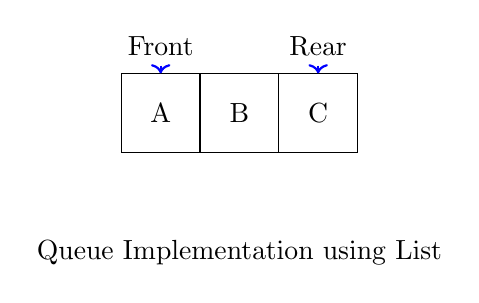
\begin{tikzpicture}[
    cell/.style={rectangle, draw, minimum size=1cm},
    ptr/.style={->, thick, blue}
]
    % Initial
    \foreach \x/\val in {0/A, 1/B, 2/C} {
        \node[cell] at (\x, 0) {\val};
    }
    \node[anchor=south] at (0, 0.6) {Front};
    \draw[ptr] (0, 0.6) -- (0, 0.5);
    \node[anchor=south] at (2, 0.6) {Rear};
    \draw[ptr] (2, 0.6) -- (2, 0.5);
    
    \node[below=1.5cm] at (1,0) {Queue Implementation using List};
\end{tikzpicture}
\captionof{figure}{Queue Implementation Pointers}
\end{center}

\begin{itemize}
    \item \textbf{Enqueue}: Add element at rear
    \item \textbf{Dequeue}: Remove element from front
    \item \textbf{FIFO principle}: First In, First Out
\end{itemize}
\end{solutionbox}

\begin{mnemonicbox}
\mnemonic{ERF - Enqueue Rear, Front}
\end{mnemonicbox}

\questionmarks{3(a)}{3}{List types of linked lists. Give graphical representation of each type.}

\begin{solutionbox}
\begin{center}
\captionof{table}{Types of Linked Lists}
\begin{tabulary}{\linewidth}{|L|L|L|}
\hline
\textbf{Type} & \textbf{Description} & \textbf{Diagram} \\ \hline
Singly & One direction pointer & $A \rightarrow B \rightarrow C \rightarrow NULL$ \\ \hline
Doubly & Two direction pointers & $NULL \leftarrow A \rightleftarrows B \rightleftarrows C \rightarrow NULL$ \\ \hline
Circular & Last points to first & $A \rightarrow B \rightarrow C \rightarrow A$ \\ \hline
\end{tabulary}
\end{center}

\begin{center}
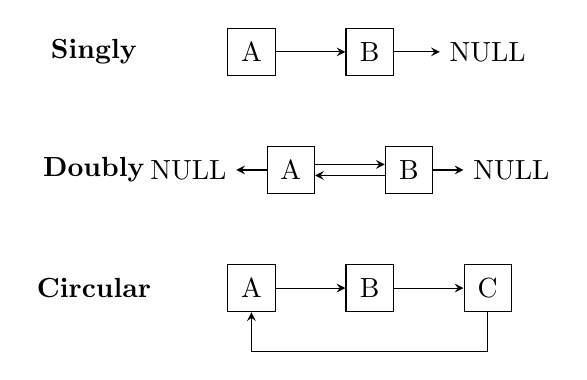
\begin{tikzpicture}[list/.style={rectangle, draw, minimum size=6mm}, >=stealth]
    % Singly
    \node (slabel) at (-2,0) {\textbf{Singly}};
    \node[list] (s1) at (0,0) {A};
    \node[list] (s2) at (1.5,0) {B};
    \node (s3) at (3,0) {NULL};
    \draw[->] (s1) -- (s2);
    \draw[->] (s2) -- (s3);

    % Doubly
    \node (dlabel) at (-2,-1.5) {\textbf{Doubly}};
    \node (dnull1) at (-0.8,-1.5) {NULL};
    \node[list] (d1) at (0.5,-1.5) {A};
    \node[list] (d2) at (2,-1.5) {B};
    \node (dnull2) at (3.3,-1.5) {NULL};
    \draw[<-] (dnull1) -- (d1);
    \draw[transform canvas={yshift=2pt}, ->] (d1) -- (d2);
    \draw[transform canvas={yshift=-2pt}, <-] (d1) -- (d2);
    \draw[->] (d2) -- (dnull2);

    % Circular
    \node (clabel) at (-2,-3) {\textbf{Circular}};
    \node[list] (c1) at (0,-3) {A};
    \node[list] (c2) at (1.5,-3) {B};
    \node[list] (c3) at (3,-3) {C};
    \draw[->] (c1) -- (c2);
    \draw[->] (c2) -- (c3);
    \draw[->] (c3.south) -- ++(0,-0.5) -| (c1.south);
\end{tikzpicture}
\captionof{figure}{Linked List Types}
\end{center}
\end{solutionbox}

\begin{mnemonicbox}
\mnemonic{SDC - Singly, Doubly, Circular}
\end{mnemonicbox}

\questionmarks{3(b)}{4}{Write an algorithm to search a given node in a singly link list.}

\begin{solutionbox}
\begin{lstlisting}[language=Python]
def search_node(head, key):
    current = head
    position = 0
    
    while current is not None:
        if current.data == key:
            return position
        current = current.next
        position += 1
    
    return -1  # Not found

# Algorithm steps:
# 1. Start from head
# 2. Compare current data with key
# 3. If found, return position
# 4. Move to next node
# 5. Repeat until end
\end{lstlisting}

\begin{itemize}
    \item \textbf{Linear search}: Traverse from head to tail
    \item \textbf{Time complexity}: O(n)
    \item \textbf{Return}: Position if found, -1 if not found
\end{itemize}
\end{solutionbox}

\begin{mnemonicbox}
\mnemonic{SCMR - Start, Compare, Move, Return}
\end{mnemonicbox}

\questionmarks{3(c)}{7}{Implement program to perform following operation on singly linked list: 1)Insert a node at the beginning of a singly linked list. 2)Delete a node from the beginning of a singly linked list.}

\begin{solutionbox}
\begin{lstlisting}[language=Python]
class Node:
    def __init__(self, data):
        self.data = data
        self.next = None

class SinglyLinkedList:
    def __init__(self):
        self.head = None
    
    def insert_at_beginning(self, data):
        new_node = Node(data)
        new_node.next = self.head
        self.head = new_node
        print(f"Inserted {data} at beginning")
    
    def delete_from_beginning(self):
        if self.head is None:
            print("List is empty")
            return None
        
        deleted_data = self.head.data
        self.head = self.head.next
        print(f"Deleted {deleted_data} from beginning")
        return deleted_data
    
    def display(self):
        current = self.head
        while current:
            print(current.data, end=" -> ")
            current = current.next
        print("NULL")
\end{lstlisting}

\begin{itemize}
    \item \textbf{Insert}: Create node, link to head, update head
    \item \textbf{Delete}: Store data, move head to next, return data
\end{itemize}
\end{solutionbox}

\begin{mnemonicbox}
\mnemonic{CLU - Create, Link, Update}
\end{mnemonicbox}

\questionmarks{3(a) OR}{3}{Differentiate between circular linked list and singly linked list.}

\begin{solutionbox}
\begin{center}
\captionof{table}{Circular vs Singly Linked List}
\begin{tabulary}{\linewidth}{|L|L|L|}
\hline
\textbf{Feature} & \textbf{Singly Linked List} & \textbf{Circular Linked List} \\ \hline
Last node points to & NULL & First node (head) \\ \hline
Traversal & Linear (one direction) & Circular (continuous) \\ \hline
End detection & next == NULL & next == head \\ \hline
Memory & Less (no extra pointer) & Same structure \\ \hline
\end{tabulary}
\end{center}
\end{solutionbox}

\begin{mnemonicbox}
\mnemonic{CNTE - Circular No Termination End}
\end{mnemonicbox}

\questionmarks{3(b) OR}{4}{Explain three applications of linked list in brief.}

\begin{solutionbox}
\begin{center}
\captionof{table}{Linked List Applications}
\begin{tabulary}{\linewidth}{|L|L|L|}
\hline
\textbf{Application} & \textbf{Description} & \textbf{Advantage} \\ \hline
\textbf{Dynamic memory allocation} & Manage memory blocks & Efficient memory usage \\ \hline
\textbf{Implementation of stacks/queues} & Using linked structure & Dynamic size \\ \hline
\textbf{Polynomial representation} & Store coefficients and powers & Easy arithmetic operations \\ \hline
\end{tabulary}
\end{center}

\begin{itemize}
    \item \textbf{Music playlist}: Add/remove songs dynamically
    \item \textbf{Browser history}: Navigate back/forward
    \item \textbf{Image viewer}: Previous/next image navigation
\end{itemize}
\end{solutionbox}

\begin{mnemonicbox}
\mnemonic{DIP - Dynamic, Implementation, Polynomial}
\end{mnemonicbox}

\questionmarks{3(c) OR}{7}{Implement a program to create and display circular linked lists.}

\begin{solutionbox}
\begin{lstlisting}[language=Python]
class Node:
    def __init__(self, data):
        self.data = data
        self.next = None

class CircularLinkedList:
    def __init__(self):
        self.head = None
    
    def insert(self, data):
        new_node = Node(data)
        
        if self.head is None:
            self.head = new_node
            new_node.next = self.head
        else:
            current = self.head
            while current.next != self.head:
                current = current.next
            current.next = new_node
            new_node.next = self.head
    
    def display(self):
        if self.head is None:
            print("List is empty")
            return
        
        current = self.head
        print("Circular List:")
        while True:
            print(current.data, end=" -> ")
            current = current.next
            if current == self.head:
                break
        print(f"{self.head.data} (back to head)")

# Example usage
cll = CircularLinkedList()
cll.insert(10)
cll.insert(20)
cll.insert(30)
cll.display()
\end{lstlisting}

\begin{itemize}
    \item \textbf{Creation}: Link last node to head
    \item \textbf{Display}: Stop when reaching head again
\end{itemize}
\end{solutionbox}

\begin{mnemonicbox}
\mnemonic{CLH - Create, Link, Head}
\end{mnemonicbox}

\questionmarks{4(a)}{3}{Write a program for Selection Sort Method.}

\begin{solutionbox}
\begin{lstlisting}[language=Python]
def selection_sort(arr):
    n = len(arr)
    
    for i in range(n):
        min_idx = i
        for j in range(i+1, n):
            if arr[j] < arr[min_idx]:
                min_idx = j
        
        arr[i], arr[min_idx] = arr[min_idx], arr[i]
    
    return arr

# Example usage
data = [64, 34, 25, 12, 22]
sorted_data = selection_sort(data)
print("Sorted array:", sorted_data)
\end{lstlisting}

\begin{itemize}
    \item \textbf{Find minimum}: In unsorted portion
    \item \textbf{Swap}: With first unsorted element
    \item \textbf{Time complexity}: $O(n^2)$
\end{itemize}
\end{solutionbox}

\begin{mnemonicbox}
\mnemonic{FMS - Find, Minimum, Swap}
\end{mnemonicbox}

\questionmarks{4(b)}{4}{Apply Insertion sort to following data to arrange them in ascending order. 25 15 35 20 30 5 10}

\begin{solutionbox}
\textbf{Insertion Sort Steps:}

\begin{center}
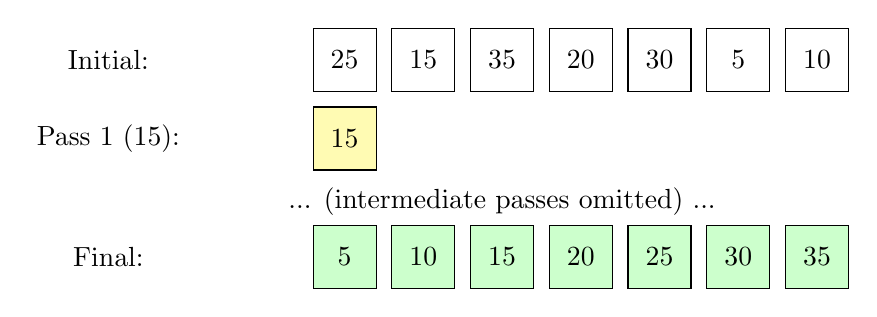
\begin{tikzpicture}[
    arrnode/.style={rectangle, draw, minimum size=0.8cm},
    highlight/.style={fill=yellow!30}
]
    % Initial
    \node (l0) at (-3, 0) {Initial:};
    \foreach \x/\val in {0/25, 1/15, 2/35, 3/20, 4/30, 5/5, 6/10} {
        \node[arrnode] at (\x, 0) {\val};
    }
    
    % Pass 1
    \node (l1) at (-3, -1) {Pass 1 (15):};
    \foreach \x/\val/\hl in {0/15/highlight, 1/25/white, 2/35/white, 3/20/white, 4/30/white, 5/5/white, 6/10/white} {
        \node[arrnode, \hl] at (\x, -1) {\val};
    }

    % Pass 6
    \node (l6) at (-3, -2.5) {Final:};
    \foreach \x/\val in {0/5, 1/10, 2/15, 3/20, 4/25, 5/30, 6/35} {
        \node[arrnode, fill=green!20] at (\x, -2.5) {\val};
    }
    
    \node at (2, -1.8) { ... (intermediate passes omitted) ... };
\end{tikzpicture}
\captionof{figure}{Insertion Sort Visualization}
\end{center}

\begin{itemize}
    \item \textbf{Method}: Take element, find position in sorted part
    \item \textbf{Comparisons}: 15 total comparisons
    \item \textbf{Shifts}: Elements moved to make space
\end{itemize}
\end{solutionbox}

\begin{mnemonicbox}
\mnemonic{TFI - Take, Find, Insert}
\end{mnemonicbox}

\questionmarks{4(c)}{7}{Implement a python program to search a particular element from a list using Linear Search.}

\begin{solutionbox}
\begin{lstlisting}[language=Python]
def linear_search(arr, target):
    comparisons = 0
    
    for i in range(len(arr)):
        comparisons += 1
        if arr[i] == target:
            print(f"Element {target} found at index {i}")
            return i
    
    print(f"Element {target} not found")
    return -1

def linear_search_all_positions(arr, target):
    positions = []
    for i in range(len(arr)):
        if arr[i] == target:
            positions.append(i)
    return positions

# Example usage
data = [10, 25, 30, 15, 20, 30, 35]
target = 30
result = linear_search(data, target)
\end{lstlisting}

\begin{itemize}
    \item \textbf{Sequential search}: Check each element one by one
    \item \textbf{Time complexity}: O(n) worst case
    \item \textbf{Best case}: O(1) if found at first position
\end{itemize}
\end{solutionbox}

\begin{mnemonicbox}
\mnemonic{CEO - Check Each One}
\end{mnemonicbox}

\questionmarks{4(a) OR}{3}{Write a program of Insertion Sort Method.}

\begin{solutionbox}
\begin{lstlisting}[language=Python]
def insertion_sort(arr):
    for i in range(1, len(arr)):
        key = arr[i]
        j = i - 1
        
        while j >= 0 and arr[j] > key:
            arr[j + 1] = arr[j]
            j -= 1
        
        arr[j + 1] = key
    
    return arr

# Example usage
data = [12, 11, 13, 5, 6]
sorted_data = insertion_sort(data.copy())
\end{lstlisting}

\begin{itemize}
    \item \textbf{Key element}: Current element to be inserted
    \item \textbf{Shift right}: Larger elements move right
    \item \textbf{Insert}: Key at correct position
\end{itemize}
\end{solutionbox}

\begin{mnemonicbox}
\mnemonic{KSI - Key, Shift, Insert}
\end{mnemonicbox}

\questionmarks{4(b) OR}{4}{Apply Quick Sort to the following data and arrange them in the proper manner. 5 6 1 8 2 9 10 15 7 13}

\begin{solutionbox}
\textbf{Quick Sort Steps:}

\begin{center}
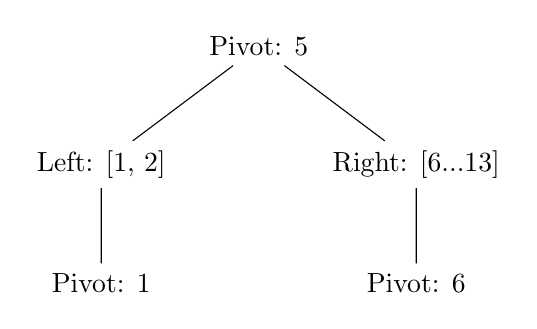
\begin{tikzpicture}[level distance=1.5cm, sibling distance=2.5cm, 
    level 1/.style={sibling distance=4cm},
    level 2/.style={sibling distance=2cm}]
    \node {Pivot: 5}
        child {node {Left: [1, 2]}
            child {node {Pivot: 1}}
        }
        child {node {Right: [6...13]}
            child {node {Pivot: 6}}
        };
\end{tikzpicture}
\captionof{figure}{Quick Sort Partitioning}
\end{center}

\begin{itemize}
    \item \textbf{Divide}: Choose pivot, partition around it
    \item \textbf{Conquer}: Recursively sort subarrays
    \item \textbf{Average time}: $O(n \log n)$
\end{itemize}
\end{solutionbox}

\begin{mnemonicbox}
\mnemonic{DCC - Divide, Conquer, Combine}
\end{mnemonicbox}

\questionmarks{4(c) OR}{7}{Implement Merge sort algorithm.}

\begin{solutionbox}
\begin{lstlisting}[language=Python]
def merge_sort(arr):
    if len(arr) <= 1:
        return arr
    
    mid = len(arr) // 2
    left = merge_sort(arr[:mid])
    right = merge_sort(arr[mid:])
    
    return merge(left, right)

def merge(left, right):
    result = []
    i = j = 0
    
    while i < len(left) and j < len(right):
        if left[i] <= right[j]:
            result.append(left[i])
            i += 1
        else:
            result.append(right[j])
            j += 1
    
    result.extend(left[i:])
    result.extend(right[j:])
    
    return result

# Example usage
data = [38, 27, 43, 3, 9, 82, 10]
sorted_data = merge_sort(data)
\end{lstlisting}

\begin{itemize}
    \item \textbf{Divide}: Split array into halves
    \item \textbf{Merge}: Combine sorted subarrays
    \item \textbf{Time complexity}: $O(n \log n)$ always
\end{itemize}
\end{solutionbox}

\begin{mnemonicbox}
\mnemonic{DSM - Divide, Sort, Merge}
\end{mnemonicbox}

\questionmarks{5(a)}{3}{Write Short note on: Applications of Tree.}

\begin{solutionbox}
\begin{center}
\captionof{table}{Tree Applications}
\begin{tabulary}{\linewidth}{|L|L|L|}
\hline
\textbf{Application} & \textbf{Description} & \textbf{Example} \\ \hline
\textbf{File systems} & Directory structure & Folders and files \\ \hline
\textbf{Expression parsing} & Mathematical expressions & $(a+b)*c$ \\ \hline
\textbf{Database indexing} & Fast data retrieval & B-trees in databases \\ \hline
\end{tabulary}
\end{center}

\begin{center}
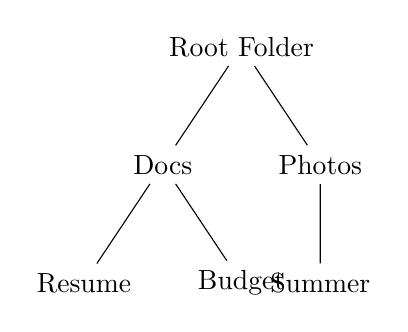
\begin{tikzpicture}[level distance=1.5cm, sibling distance=2cm]
    \node {Root Folder}
        child {node {Docs}
            child {node {Resume}}
            child {node {Budget}}
        }
        child {node {Photos}
            child {node {Summer}}
        };
\end{tikzpicture}
\captionof{figure}{File System Tree Structure}
\end{center}

\begin{itemize}
    \item \textbf{Decision trees}: AI and machine learning
    \item \textbf{Huffman coding}: Data compression
    \item \textbf{Game trees}: Chess, tic-tac-toe
\end{itemize}
\end{solutionbox}

\begin{mnemonicbox}
\mnemonic{FED - File, Expression, Database}
\end{mnemonicbox}

\questionmarks{5(b)}{4}{Explain different Tree Traversal Methods.}

\begin{solutionbox}
\begin{center}
\captionof{table}{Tree Traversal Methods}
\begin{tabulary}{\linewidth}{|L|L|L|}
\hline
\textbf{Method} & \textbf{Order} & \textbf{Process} \\ \hline
\textbf{Inorder} & Left-Root-Right & LNR \\ \hline
\textbf{Preorder} & Root-Left-Right & NLR \\ \hline
\textbf{Postorder} & Left-Right-Root & LRN \\ \hline
\end{tabulary}
\end{center}

\begin{center}
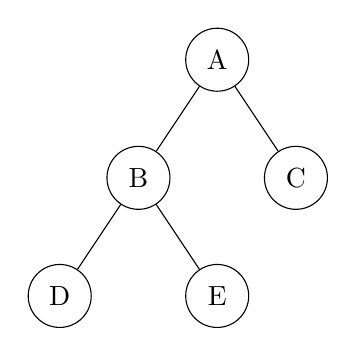
\begin{tikzpicture}[level distance=1.5cm, sibling distance=2cm, nodes={circle, draw, minimum size=0.8cm}]
    \node {A}
        child {node {B}
            child {node {D}}
            child {node {E}}
        }
        child {node {C}};
\end{tikzpicture}
\captionof{figure}{Example Tree for Traversal}
\end{center}

\begin{itemize}
    \item \textbf{Inorder}: D B E A C (Left, Root, Right)
    \item \textbf{Preorder}: A B D E C (Root, Left, Right)
    \item \textbf{Postorder}: D E B C A (Left, Right, Root)
\end{itemize}
\end{solutionbox}

\begin{mnemonicbox}
\mnemonic{LNR PNL LRN for In-Pre-Post}
\end{mnemonicbox}

\questionmarks{5(c)}{7}{Write a menu driven program to perform the following operation on Binary Search Tree: Create a BST.}

\begin{solutionbox}
\begin{lstlisting}[language=Python]
class TreeNode:
    def __init__(self, data):
        self.data = data
        self.left = None
        self.right = None

class BST:
    def __init__(self):
        self.root = None
    
    def insert(self, data):
        self.root = self._insert_recursive(self.root, data)
    
    def _insert_recursive(self, node, data):
        if node is None:
            return TreeNode(data)
        
        if data < node.data:
            node.left = self._insert_recursive(node.left, data)
        elif data > node.data:
            node.right = self._insert_recursive(node.right, data)
        
        return node
    
    def inorder(self, node):
        if node:
            self.inorder(node.left)
            print(node.data, end=" ")
            self.inorder(node.right)

def main():
    bst = BST()
    while True:
        print("\n1. Insert")
        print("2. Display (Inorder)")
        print("3. Exit")
        choice = int(input("Enter choice: "))
        if choice == 1:
            data = int(input("Enter data: "))
            bst.insert(data)
        elif choice == 2:
            print("BST (Inorder):", end=" ")
            bst.inorder(bst.root)
            print()
        elif choice == 3:
            break

if __name__ == "__main__":
    main()
\end{lstlisting}

\begin{itemize}
    \item \textbf{BST property}: Left < Root < Right
    \item \textbf{Insertion}: Compare and go left/right
\end{itemize}
\end{solutionbox}

\begin{mnemonicbox}
\mnemonic{CIM - Compare, Insert, Menu}
\end{mnemonicbox}

\questionmarks{5(a) OR}{3}{Define and give examples : Strict Binary Tree and Complete Binary Tree.}

\begin{solutionbox}
\begin{center}
\captionof{table}{Binary Tree Types}
\begin{tabulary}{\linewidth}{|L|L|L|}
\hline
\textbf{Type} & \textbf{Definition} & \textbf{Example} \\ \hline
\textbf{Strict Binary Tree} & Every node has 0 or 2 children & Internal nodes have 2 children \\ \hline
\textbf{Complete Binary Tree} & Levels filled except last (L to R) & Perfect structure till 2nd last \\ \hline
\end{tabulary}
\end{center}

\begin{center}
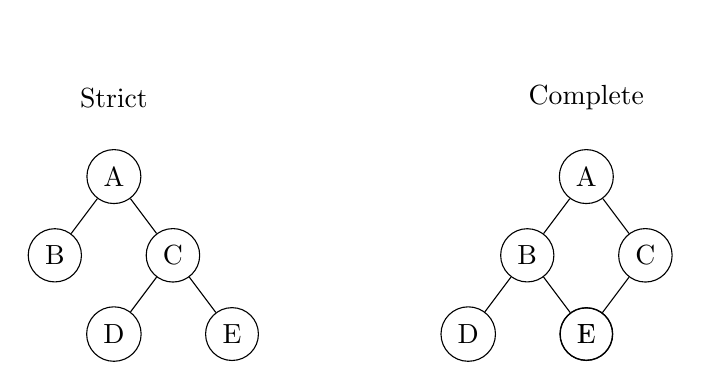
\begin{tikzpicture}[level distance=1cm, sibling distance=1.5cm, nodes={circle, draw, minimum size=0.6cm}]
    % Strict
    \node at (-3, 1) [draw=none] {Strict};
    \node at (-3, 0) {A}
        child {node {B}}
        child {node {C}
            child {node {D}}
            child {node {E}}
        };

    % Complete
    \node at (3, 1) [draw=none] {Complete};
    \node at (3, 0) {A}
        child {node {B}
            child {node {D}}
            child {node {E}}
        }
        child {node {C}
            child {node {F}}
            child[missing]
        };
\end{tikzpicture}
\captionof{figure}{Binary Tree Types}
\end{center}
\end{solutionbox}

\begin{mnemonicbox}
\mnemonic{SC - Strict Complete}
\end{mnemonicbox}

\questionmarks{5(b) OR}{4}{Explain basic terminology of Binary Tree : Level number, Degree, Indegree , Out-degree , Leaf Node.}

\begin{solutionbox}
\begin{center}
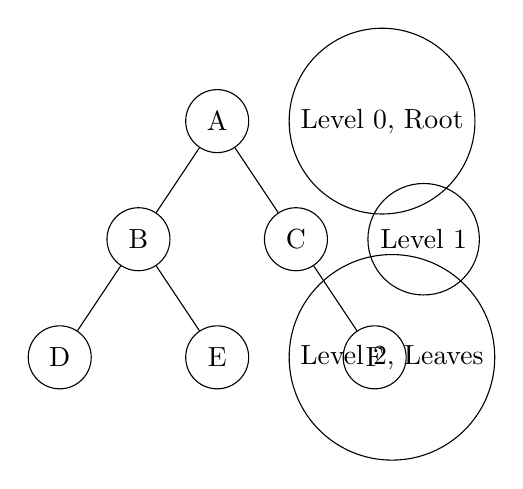
\begin{tikzpicture}[level distance=1.5cm, sibling distance=2cm, nodes={circle, draw, minimum size=0.8cm}]
    \node (A) {A}
        child {node (B) {B}
            child {node (D) {D}}
            child {node (E) {E}}
        }
        child {node (C) {C}
            child [missing]
            child {node (F) {F}}
        };
    
    \node[right=0.5cm of A] {Level 0, Root};
    \node[right=2.5cm of B] {Level 1};
    \node[right=2.5cm of D] {Level 2, Leaves};
\end{tikzpicture}
\captionof{figure}{Binary Tree Terminology}
\end{center}

\begin{center}
\captionof{table}{Binary Tree Terminology}
\begin{tabulary}{\linewidth}{|L|L|L|}
\hline
\textbf{Term} & \textbf{Definition} & \textbf{Example} \\ \hline
\textbf{Level number} & Distance from root (root = 0) & A=0, B=1, D=2 \\ \hline
\textbf{Degree} & Number of children & A=2, B=2, C=1 \\ \hline
\textbf{Indegree} & Number of incoming edges & All nodes = 1 (except root = 0) \\ \hline
\textbf{Out-degree} & Number of outgoing edges & Same as degree \\ \hline
\textbf{Leaf Node} & Node with no children & D, E, F \\ \hline
\end{tabulary}
\end{center}
\end{solutionbox}

\begin{mnemonicbox}
\mnemonic{LDIOL - Level, Degree, In-Out, Leaf}
\end{mnemonicbox}

\questionmarks{5(c) OR}{7}{Write a menu driven program to perform the following operation on Binary Search Tree: Insert an element in BST.}

\begin{solutionbox}
\begin{lstlisting}[language=Python]
class TreeNode:
    def __init__(self, data):
        self.data = data
        self.left = None
        self.right = None

class BST:
    def __init__(self):
        self.root = None
    
    def insert(self, data):
        if self.root is None:
            self.root = TreeNode(data)
            print(f"Root node {data} created")
        else:
            self._insert_helper(self.root, data)
    
    def _insert_helper(self, node, data):
        if data < node.data:
            if node.left is None:
                node.left = TreeNode(data)
                print(f"Inserted {data} to left of {node.data}")
            else:
                self._insert_helper(node.left, data)
        elif data > node.data:
            if node.right is None:
                node.right = TreeNode(data)
                print(f"Inserted {data} to right of {node.data}")
            else:
                self._insert_helper(node.right, data)
        else:
            print(f"Data {data} already exists")

    def display_inorder(self, node, result):
        if node:
            self.display_inorder(node.left, result)
            result.append(node.data)
            self.display_inorder(node.right, result)

# ... (Main function same as above)
\end{lstlisting}

\begin{itemize}
    \item \textbf{Insert logic}: Compare with current node, go left/right
    \item \textbf{Recursive approach}: Clean and efficient implementation
\end{itemize}
\end{solutionbox}

\begin{mnemonicbox}
\mnemonic{CRL - Compare, Recursive, Left/right}
\end{mnemonicbox}

\end{document}
